%%%%%%%%%%%%%%%%%%%%%%%%%%%%%%%%%%%%%%%%%%%%%%%%%%%%%%%%%%%%%%%%
% %
% Due Date %
% Andrew Gibson %
% ECE 351 lab, Section 53 %
% Lab 10 %
% Due 25 April 2023 %
% Fast Fourier Transform %
% https://github.com/gibs0630/ECE351\_Code %
% https://github.com/gibs0630/ECE351\_Reports %
% %
%%%%%%%%%%%%%%%%%%%%%%%%%%%%%%%%%%%%%%%%%%%%%%%%%%%%%%%%%%%%%%%%

\documentclass[12pt,a4paper]{article}
\usepackage[utf8]{inputenc}
\usepackage[greek,english]{babel}
\usepackage{alphabeta} 
\usepackage[pdftex]{graphicx}
\usepackage[top=1in, bottom=1in, left=1in, right=1in]{geometry}
\linespread{1.06}
\setlength{\parskip}{8pt plus2pt minus2pt}
\widowpenalty 10000
\clubpenalty 10000
\newcommand{\eat}[1]{}
\newcommand{\HRule}{\rule{\linewidth}{0.5mm}}
\usepackage[official]{eurosym}
\usepackage{enumitem}
\setlist{nolistsep,noitemsep}
\usepackage[hidelinks]{hyperref}
\usepackage{cite}
\usepackage{lipsum}

\newcommand{\Q}{\leavevmode\par\textbf {Q:}}
\newcommand{\A}{\par\textbf{A:} \normalfont}

\hypersetup{colorlinks=true, linkcolor=black, urlcolor=blue}

\begin{document}
%===========================================================
\begin{titlepage}
\begin{center}
% Top 
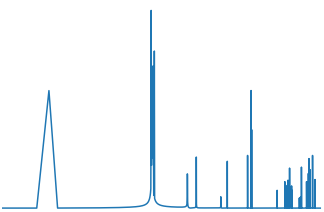
\includegraphics[width=0.55\textwidth]{titlepage_image.png}~\\[2cm]
% Title
\HRule \\[0.4cm]
{ \LARGE 
  \textbf{Project Report for ECE 351}\\[0.4cm]
  \emph{Lab Final: Filter Design}\\[0.4cm]
}
\HRule \\[1.5cm]
% Author
{ \large
  Andrew Gibson \\[0.1cm]
 24 April 2023\\[0.1cm]
  \url{https://github.com/gibs0630/ECE351\_Code}\\[0.1cm]
  \url{https://github.com/gibs0630/ECE351\_Reports}\\[0.1cm]
  %#\texttt{user@cut.ac.cy}
}
\vfill
%\textsc{\Large Cyprus University of Technology}\\[0.4cm]\textsc{\large Department of Electrical Engineering,\\Computer Engineering \& Informatics}\\[0.4cm]
% Bottom
{\large }
 
\end{center}
\end{titlepage}
%\begin{abstract}
%\lipsum[1-2]
%\addtocontents{toc}{\protect\thispagestyle{empty}}
%\end{abstract}
\newpage
%===========================================================
\tableofcontents
\addtocontents{toc}{\protect\thispagestyle{empty}}
\newpage
\setcounter{page}{1}
%===========================================================
%===========================================================
\section{Introduction}\label{sec:intro}
With Python, it is possible to design a filter so that only a specific signal passes through.  A signal from a sensor can be operated in a variety of locations with different noise profile and filters may need to be used to only get the desired sensor data and nothing else for a particular input.  A band-pass filter can be used to do this operation.

\section{Equations}\label{sec:lit-rev}
Formula's used

Bandpass filter
\[ \frac {K bw s} {s^2 + bw*s + w_0^2} \]
\[\frac{\frac{R}{L} s} {s^2 + \frac{R}{L} s + \frac{1}{LC}}\]



\section{Methodology}\label{sec:meth}
This lab had us design a band-pass filter that had certain gain characteristics for certain frequency ranges.  First was to conduct a Laplace transform and identify the noise. Luckily, the frequencies near the signal were clear, allowing for high attenuation where noise was occurring without having to worry as much on noise near the signal frequency surviving through the desired filter.  On the higher frequency side, the band-pass filter was not actually able to attain the criteria of the desired attenuation even for a wider range of bandwidths (bw) and center frequencies ($\omega_0$) were checked through brute force methods. However, the remaining noise that wasn't properly attenuated was less than 0.05V, and was assumed to be negligible. A 1k $\Omega$ resistor was then selected arbitrarily, and potential capacitor and inductor were calculated accordingly.

\section{Results}\label{sec:res}
\subsection*{Part 1}


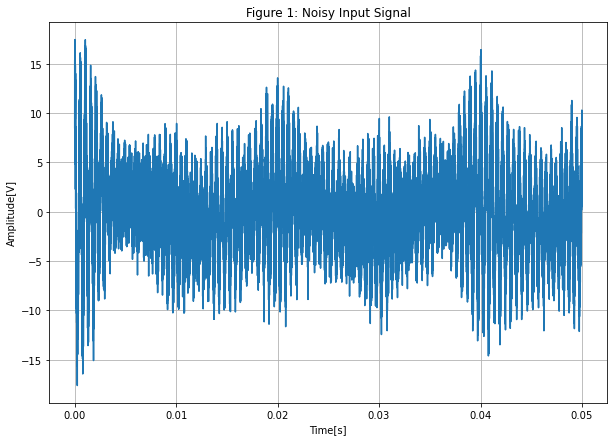
\includegraphics[width=0.8\textwidth]{Figure 1.png}\\
Figure 1 shows the original signal as captured from an oscilloscope. \\


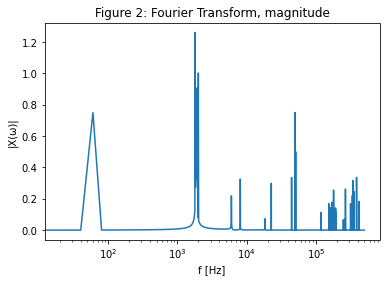
\includegraphics[width=0.8\textwidth]{Figure 2.png}\\
Figure 2 shows the magnitude of the signal, clearly showing the data signal and the noise.\\


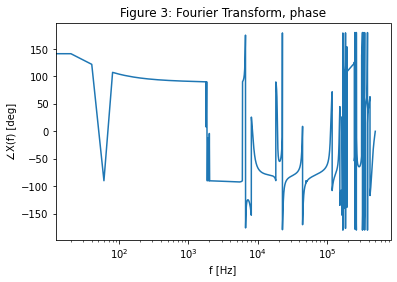
\includegraphics[width=0.8\textwidth]{Figure 3.png}\\
Figure 3 shows the phase of the signal.\\

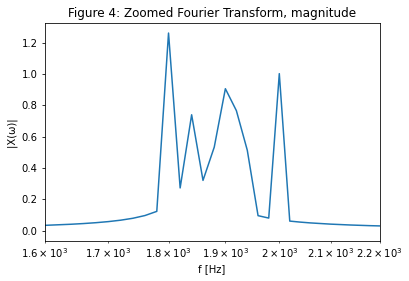
\includegraphics[width=0.8\textwidth]{Figure 4.png}\\
Figure 4 shows the zoomed in of the magnitude of sensor data between 1800 Hz and 2000 Hz.\\

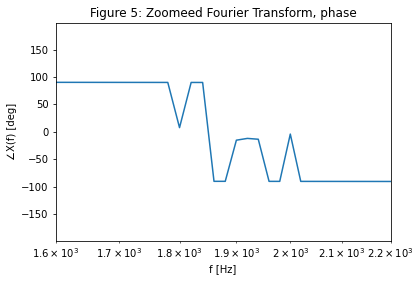
\includegraphics[width=0.8\textwidth]{Figure 5.png}\\
Figure 5 shows the zoomed in of the phase of the sensor data between 1800 Hz and 2000 Hz.\\


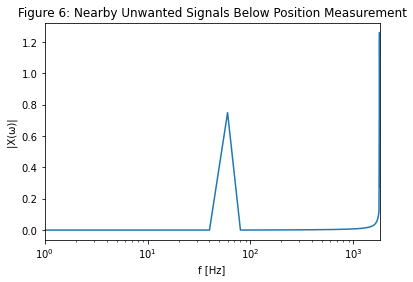
\includegraphics[width=0.8\textwidth]{Figure 6.png}\\
Figure 6 shows the nearest noise on the low frequency side, and we can see that there is a noise source at 60 Hz, which was identified to be from ventilation.\\


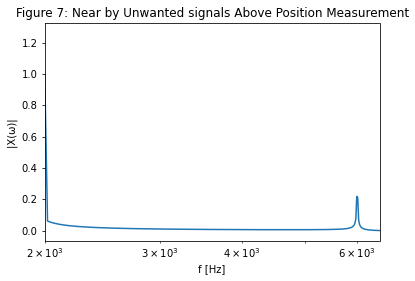
\includegraphics[width=0.8\textwidth]{Figure 7.png}\\
Figure 7 shows the nearest noise on the high frequency side of the sensor signal, and we can see the noise source at 6000 Hz, which was identified to be from switching amplifier.\\


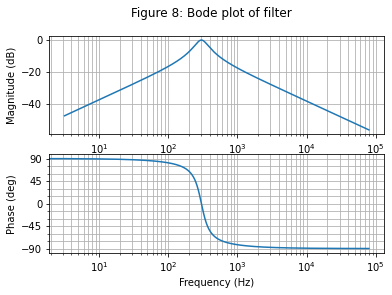
\includegraphics[width=0.8\textwidth]{Figure 8.png}\\
Figure 8 shows the bode plot of the filter which as designed by selecting the center frequency and increasing the BW until more criteria was reached.\\


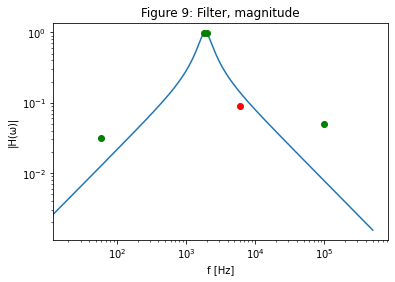
\includegraphics[width=0.8\textwidth]{Figure 9.png}\\
Figure 9 shows the which criteria failed. The first criteria was the sensor data was to not to be attenuated below -0.3 dB, which was attained at $\omega_0$ = 1900 Hz and BW = 769 Hz, which are the two overlapping green dots at the peak. The second criteria was that the low frequency noise was attenuated below -30 dB, which was the left most green dot. The third criteria was that the high frequency that was to be attenuated below -21 dB and was not attained, which is the red dot. the final criteria was that frequencies above 100 kHz were to be attenuated out completely with less than 0.05V after filtering, and is green circle on the right.\\


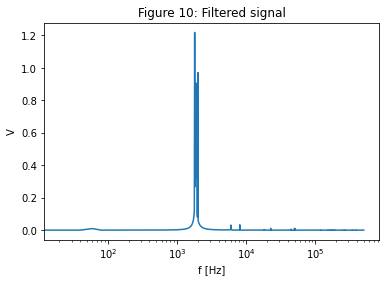
\includegraphics[width=0.8\textwidth]{Figure 10.png}\\
Figure 10 shows the magnitude signal after being passed through the filter, some of the noise has still made it through.\\


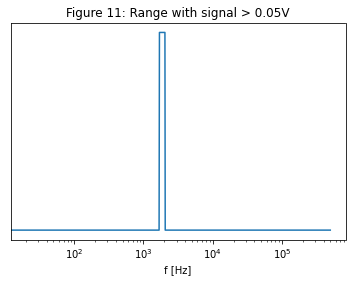
\includegraphics[width=0.8\textwidth]{Figure 11.png}\\
Figure 11 shows which signal range was above 0.05V, and the perceived noise as seen from figure 10 can be ignored according to the fourth criteria.\\


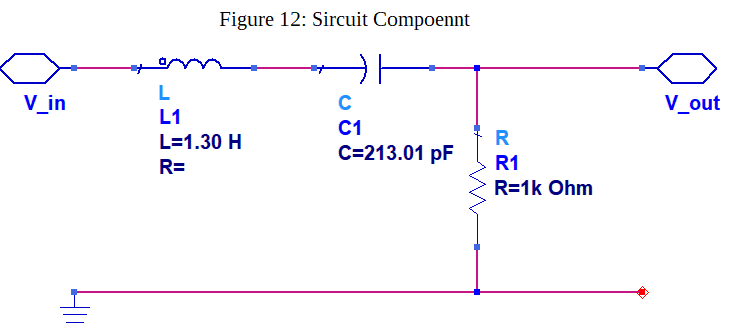
\includegraphics[width=0.8\textwidth]{Figure 12.png}\\
Figure 12 shows the schematic of the circuit to be constructed. so that the filter does not have to happen digitally. the values of the capacitor and inductor are rounded; more accurate value of the capacitor is C = 2.1301939058171745152354570637119e-7 F, and a more accurate value of the inductor is L = 1.3003901170351105331599479843953 H \\



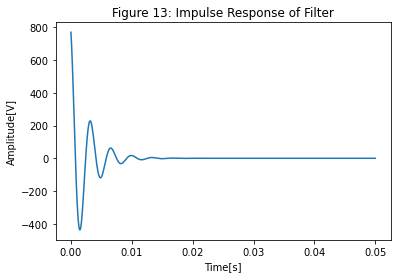
\includegraphics[width=0.8\textwidth]{Figure 13.png}\\
Figure 13 shows the impulse response of the designed circuit\\

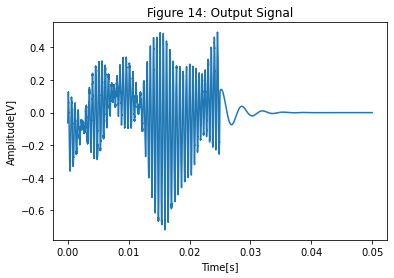
\includegraphics[width=0.8\textwidth]{Figure 14.png}\\
Figure 14 show the signal after going through the filter. because of the high frequency of 1800 Hz to 2000 Hz, not all intricacies of the sensor waveform could be captured in the figure.\\



\section{Questions}\label{sec:res}

\Q Earlier this semester, you were asked what you personally wanted to get out of taking this course. Do you feel like that personal goal was met? Why or why not?
\A I have met my goals of getting some exploration on applications and a passing class.  I know how to create a program that will do digital filtering.

\Q Please fill out the course feedback survey, I will read every word and very much appreciate the feedback.
\A It is done.

\Q  Good luck in the rest of your education and career!
\A  Thank you.



\section{Conclusion}\label{sec:res}
Using simulation it is easier to check if a circuit will behave similar to a physical device without the need to construct it immediately. This allows for checking adjacent parameters that could be expensive to conduct with hardware. Using Python, the whole process to design a filter can be streamlined.


%\lipsum[7-8]\cite{knuthwebsite}
%===========================================================
%===========================================================
\bibliographystyle{ieeetr}
\bibliography{refs}
\end{document} 
Annotations











